\begin{figure}[h!]
    \centering
   \captionsetup[sub]{font=small}
    \begin{minipage}[h!]{1\textwidth}
        \begin{subfigure}[b!]{1 \textwidth}
            \caption{}
            \vspace*{-2em}
            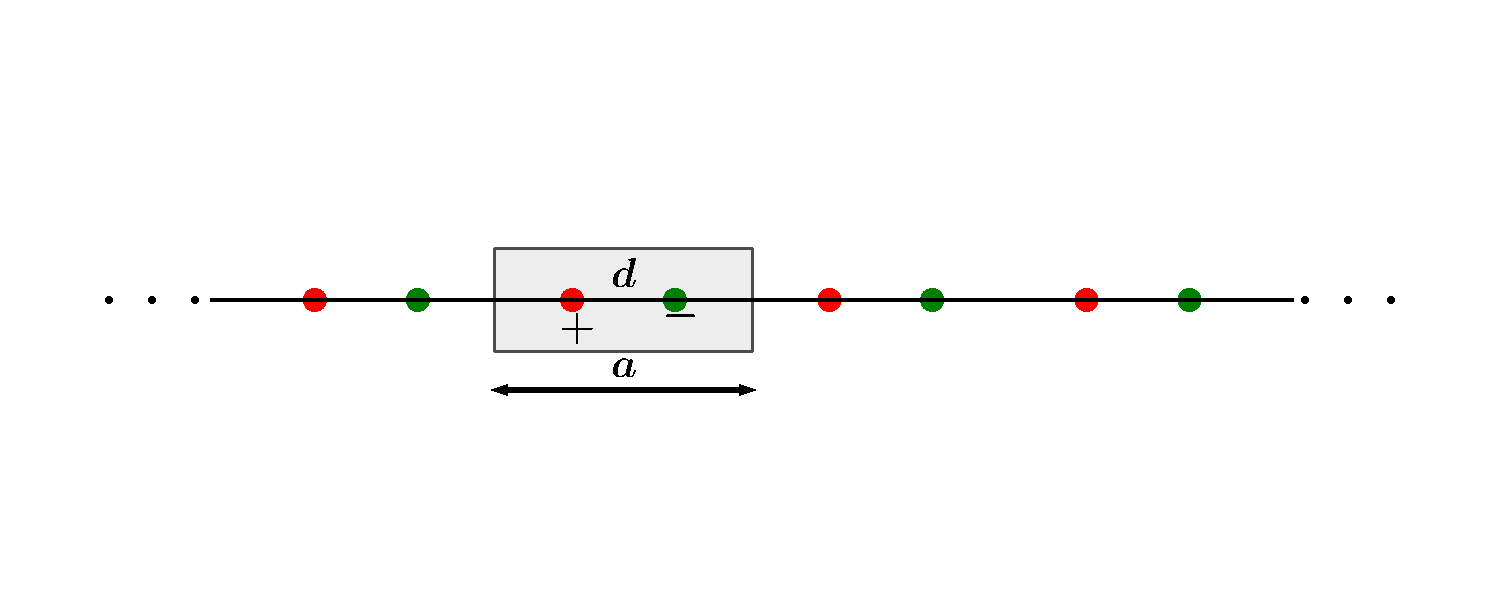
\includegraphics[width=\textwidth]{Imagenes/Models/polarizatio_example_a.pdf}
        \end{subfigure}\hspace*{-0.5em}
    \end{minipage}\vspace*{-2.5em}

    \begin{minipage}[h!]{1\textwidth}
        \begin{subfigure}[b!]{1 \textwidth}
            \caption{}
            \vspace*{-2em}
            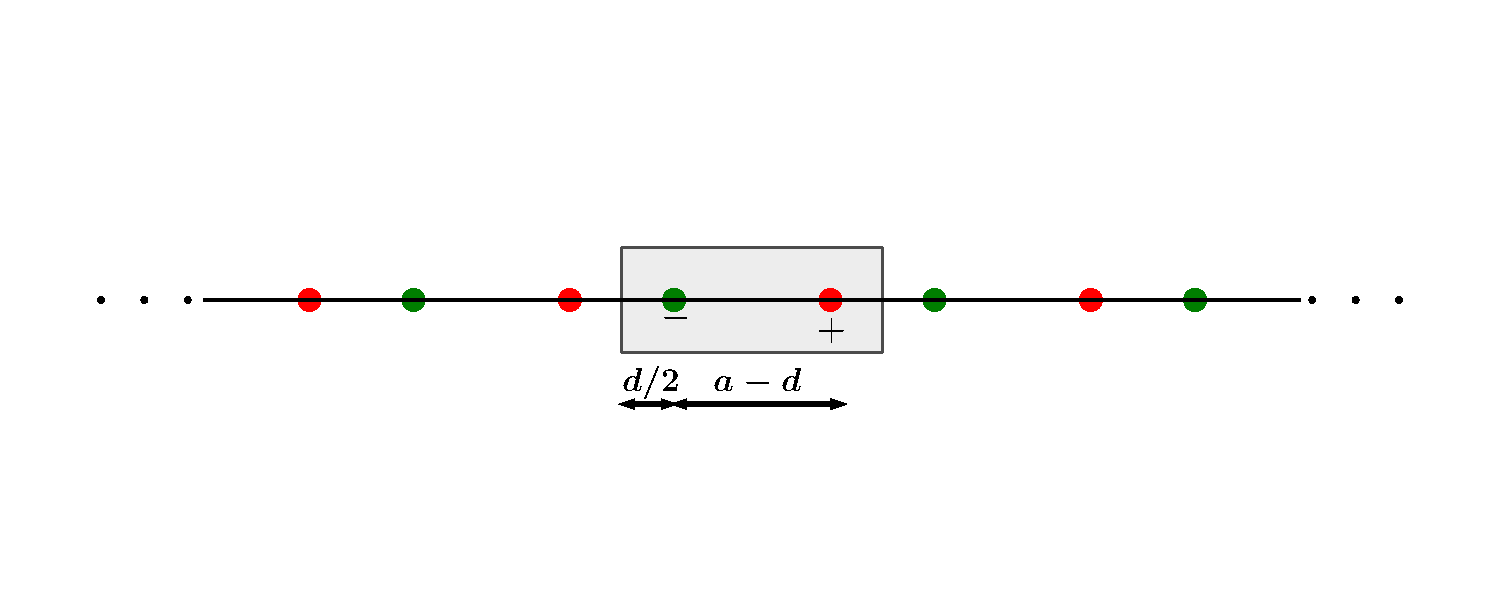
\includegraphics[width=\textwidth]{Imagenes/Models/polarizatio_example_b.pdf}
        \end{subfigure}\hspace*{-0.5em}
    \end{minipage}\vspace*{-1.5em}
    
    \caption{Red cristalina infinita periódica conformada por una molécula dicotómica anión (verde), catión (rojo), separados por una distancia \textbf{(a)} $d$ o \textbf{(b)} $a-d$, dependiendo la elección de celda.}
    \label{fig:Model_polarization}
\end{figure}